% =====================================================================
%  Chapter 14 — The Verdict, Part II
% =====================================================================

\chapter{A Protocol for Settling This}
\label{ch:protocol}

A finding of ``formally certified, mathematically unaudited'' is only useful
if it comes with a way to complete the second half. This chapter gives one,
in the order a careful reader should actually work, with the commands where
they exist and the reading tasks where they do not.

The protocol is not a contribution to the mathematics. It is a work plan, and
its purpose is to make the remaining work finite and checkable.

\begin{seamnote}{What has already been done}
Phases 1 and 2 below were completed by the community on 20 and 21 November
2026, and the results are public: the development compiles, the axiom list is
the three standard ones, the exported proof is accepted by Lean's kernel and
by independently implemented checkers, and the theorem proved has been matched
against Mathlib's \texttt{RiemannHypothesis} by two independent tools. The
commands are given anyway, because a protocol that has been run once should
be runnable again, and because a reader reproducing them is doing something
the certification does not do for them.

Phase 3 is the phase that has not been done, and it is the phase that decides
the mathematics. It is the only phase this book insists on.
\end{seamnote}

\section{Phase 1: mechanical (hours to days)}\subsection{Build}\begin{seamnote}{Commands}
\begin{leanquote}
git clone <the author's distribution, or the mirror>
cd lean
elan toolchain install $(cat lean-toolchain)
lake exe cache get
lake build Main
\end{leanquote}
The cache step matters: it fetches Mathlib's prebuilt \texttt{.olean} files
for the pinned revision, which turns the dependency from a multi-hour compile
into a download. This book's own attempt confirmed that the pinned revision
\code{0df444a360eaa60ab8c11dca51a86af692955474} is available from the
community cache.
\end{seamnote}

Record the elapsed time and peak memory. The mirror's README notes that no
build time or memory figures have been published; a reader who publishes them
does the next reader a genuine service.

\subsection{Axioms}\begin{seamnote}{Commands}
\begin{leanquote}
# in a scratch file importing the submission
import Main
#print axioms Main.riemannHypothesis
#print axioms Main.riemannZeta_eq_zero_re
#print axioms Main.LFunction_ne_zero_of_half_lt_re
#print axioms Main.LFunction_eq_zero_re
#print axioms Main.LFunction_eq_zero_re_of_isPrimitive
\end{leanquote}
\end{seamnote}

The expected output is exactly:

\begin{leanquote}
'Main.riemannHypothesis' depends on axioms: [propext, Classical.choice, Quot.sound]
\end{leanquote}

and the same for the other four. Anything else --- \texttt{sorryAx},
\texttt{Lean.ofReduceBool}, a custom axiom --- is a finding, and a
disqualifying one.

\subsection{Independent kernel replay}This step exists to remove the elaborator from the trust chain. The toolchain
is \texttt{lean4export}\idx{lean4export} to export the compiled environment, an independent
kernel implementation such as NanoDa\idx{NanoDa} to re-check it, and \texttt{landrun} to
run Lean in a sandbox. \texttt{lean4checker} provides a third-party route to
the same assurance. The Lean FRO documents these tools; they are cited in the
arXiv literature as ``Lean FRO, 2025/2026''.

\begin{seamnote}{Commands (indicative)}
\begin{leanquote}
lake exe export .olean Main.olean > main.json
# then check main.json with an external kernel, e.g.
#   python3 -m lean4checker main.json
# or with a NanoDa-based harness
\end{leanquote}
The exact invocation depends on the tool's current interface; check the
tool's own documentation rather than trusting this sketch.
\end{seamnote}

\subsection{Re-run the static scan}\begin{seamnote}{Commands}
\begin{leanquote}
rg --no-ignore -c '^\s*axiom\s' -g '*.lean' . | wc -l
rg --no-ignore -c '\bsorry\b' -g '*.lean' . | wc -l
rg --no-ignore -c '\badmit\b' -g '*.lean' . | wc -l
rg --no-ignore -c '\bnative_decide\b' -g '*.lean' . | wc -l
rg --no-ignore -c '^\s*opaque\s' -g '*.lean' . | wc -l
rg --no-ignore -n '\baddDecl\b' -g '*.lean' .
rg --no-ignore -n 'maxHeartbeats 0' -g '*.lean' .
rg --no-ignore -l '\b(elab|macro|syntax)\b' -g '*.lean' .
\end{leanquote}
Compare with \tabref{tab:scan}. Any disagreement with the published scan
should be resolved before going further, since a disagreement means one of
the two scans is wrong about something.
\end{seamnote}

\section{Phase 2: the structural trace (days)}\subsection{Confirm the chain}Walk the eight links of Chapter~7 in the source and confirm that each
declaration is present, with the statement quoted there, and that each proof
term is what the book says it is. This is cheap and it protects against the
possibility that the version you downloaded is not the version that was
announced.

\subsection{Confirm the statement is Mathlib's}\begin{seamnote}{Commands}
\begin{leanquote}
grep -n "def RiemannHypothesis" \
  .lake/packages/mathlib/Mathlib/NumberTheory/LSeries/RiemannZeta.lean
grep -n "def riemannZeta" \
  .lake/packages/mathlib/Mathlib/NumberTheory/LSeries/RiemannZeta.lean
\end{leanquote}
Both should come back with \texttt{Mathlib}'s own definitions. The mirror
records \texttt{RiemannHypothesis} at line 185 and \texttt{riemannZeta} at
line 121 at the pinned commit.
\end{seamnote}

This is the single most important check in the whole protocol, because it is
the one that cannot be got wrong in a way that is hard to detect. If
\texttt{riemannZeta} in the top-level theorem is not Mathlib's, the artifact
proves nothing about the Riemann hypothesis no matter how clean it is.

\section{Phase 3: statement review (weeks to months)}This is the phase that has not been done, and the phase that decides the
question. It cannot be automated, and this book cannot do it, because it
requires comparing the formalized statements against the published literature
in four substantial fields.

\subsection{Step 1: the automorphy bundle}Read \code{UpperTheory.V.Af.Hypotheses\_2} field by field against the
published statements.

\begin{description}[style=nextline,leftmargin=0pt,labelwidth=0pt,labelsep=0pt,font=\sffamily\bfseries\small,
  itemsep=5pt]
\item[\texttt{conjC : ClozelConjC}.] The formal statement is a specific
mathematical assertion about conjugate algebraicity of cuspidal
representations. Locate Clozel's published statement and compare quantifier
by quantifier. In particular: is the formal statement a \emph{consequence} of
published results, as the derivation chain
\texttt{clozelConjC\_of\_steps} suggests, and if so, is the chain sound? The
chain's components are named in the source and each has its own file; the
question is whether each is the classical theorem.
\item[\texttt{borelC : BorelInjC}.] Borel injectivity is proved in many cases
and conjectured in general. \emph{Which cases does the formalized statement
cover?} If it is stated for all $E$ and all $a$ without restriction, and the
classical result is restricted, that is a finding.
\item[\code{gkR : GelfandKazhdanReal}.] Compare against the Gelfand--Kazhdan
correspondence for $\mathrm{GL}_2$.
\item[\texttt{newform : NewformRep}.] This is the field that supplies the
automorphic representation. \emph{What exactly does it assert?} It is the
modularity input, and its content determines whether the automorphy step is a
theorem or a transfer.
\item[\texttt{galR}, \texttt{smoR}, \texttt{bc}.] Base change and the strong
multiplicity-one property for $\mathrm{GL}_2$; compare with the published
statements.
\end{description}

\subsection{Step 2: the admissibility and vanishing packages}Trace where instances of \code{GlobalTheory.Ord2.admitted} are
\emph{constructed}, as opposed to assumed. The structure has seven fields:
continuity, determinant $\pm 1$, oddness, irreducibility, level away from $l$,
modularity with a newform and an attached character, and the flag condition.
Each field is a real mathematical condition. The question is whether the
instances satisfy them, and where the newform in the \texttt{modular} field
comes from.

Then check the application of \texttt{VanishOrd}: the Selmer-vanishing
statement is applied to representations that are admitted; is it applied in a
setting where the hypotheses of the underlying Iwasawa-theoretic theorem
hold?

\subsection{Step 3: the theta lift}Read \texttt{UpperTheory.TP.TLiftK} against the classical theta-lift
existence statement, and then read the twenty components of
\code{UpperTheory.TP.Tools\_k} --- in particular
\texttt{siegelWeilAniso\_of\_k}, \texttt{epsOf\_of\_k}, and
\texttt{hgtEx\_of\_k} --- against the theorems they are named for.

\subsection{Step 4: the applications}The hardest part, and the one that no mechanical check can help with. A
faithful formalisation of a classical theorem can still be \emph{applied}
where the classical theorem does not apply: at a prime that ramifies, to a
representation that is not cuspidal, to a lift outside the orthogonal
complement, at a place that the argument assumes is unramified but is not.

\subsection{Step 5: the remark against the code}Finally, return to the remark with the code in hand and ask the two questions
the remark refuses to answer:

\begin{quote}
\textbf{Question 1.} Item 14 says the method would stop at 2/3 a priori, and
item 20 says GRH the next day. \emph{Where in the development is the step
that crosses the ceiling?} If it can be located, the question is answered. If
it cannot be located, that is the most important negative finding available,
and it should be published.

\textbf{Question 2.} Item 17 says the $H^1_o$ classes not killed by twisting
require a significant weakening of Vandiver. \emph{Is there a formalized
statement corresponding to that weakening, and is it proved?} If yes, the
author has proved something nobody has. If no, then item 17 describes an
obstacle the artifact does not remove.
\end{quote}

\begin{figure}[!htbp]
\centering
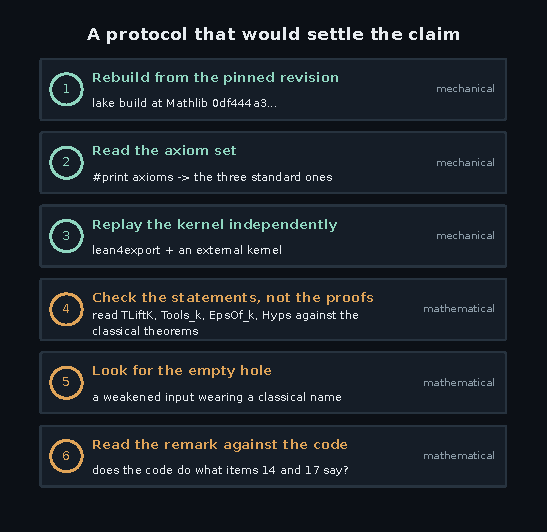
\includegraphics[width=\textwidth]{../figures/fig_protocol.pdf}
\caption{The protocol, in order. The first three steps are mechanical and
have effectively been done. The last three are mathematical, have not been
done, and are the ones that decide the question.}
\label{fig:protocol}
\end{figure}

\section{What a result at each step would mean}\begin{table}[H]
\centering
\caption{Outcomes.}
\label{tab:outcomes}
\begin{tabular}{@{}>{\RaggedRight\arraybackslash\hyphenpenalty=10000\exhyphenpenalty=10000}p{0.28\textwidth}>{\RaggedRight\arraybackslash\hyphenpenalty=10000\exhyphenpenalty=10000}p{0.56\textwidth}@{}}
\toprule
\textbf{Step} & \textbf{If it succeeds} \\
\midrule
Build & The artifact is complete and reproducible. Confirms the claim of
October--November 2026 on a third machine. \\
Axiom check & The formal layer is sound. Removes the crudest hypotheses from
consideration. \\
Kernel replay & The result does not depend on the elaborator or on the
repository's metaprogramming. \\
Statement review & \textbf{The claim is settled, in one direction or the
other.} This is the step that matters. \\
\bottomrule
\end{tabular}
\end{table}

It is worth being explicit that a statement review could \emph{refute} the
claim. If a reader finds that \texttt{ClozelConjC} as formalized is strictly
weaker than Clozel's published statement, or that the instances of
\texttt{admitted} are not constructed but assumed, the chain breaks, and the
result would be a negative finding about the artifact rather than about the
Riemann hypothesis. That would be a valuable outcome, and it is the kind of
outcome that only a review can produce.

\begin{keytakeaways}

\item Phase 1 --- build, axiom check, kernel replay, static scan --- is
mechanical, and it was completed by the community on 20 and 21 November 2026,
with the results and logs public.
\item Phase 2 --- confirming the chain and confirming that the statement is
Mathlib's --- was also completed: the statement comparison was done by two
independent tools, and this book independently confirms the chain and the
archive's checksum.
\item Phase 3 --- statement review of the five load-bearing inputs, their
applications, and the remark against the code --- is weeks to months of
specialist work, and it is the step that decides the question.
\item A successful review could refute the claim as well as confirm it. That
is what makes it worth doing.
\end{keytakeaways}
